%%%%Select the class of document
\documentclass{amsart} %type/class of article
%\documentclass{article}
%\documentclass{book}
%\documentclass{letter}

%%%%Select packages
\usepackage{amsthm,amsmath,amssymb} %math packages (always include)
\usepackage{geometry} %can be used to modify page dimensions, etc.
\usepackage{graphicx} %figure
\usepackage{float} %figure position in pdf
\usepackage{multirow} %table with multirow
\usepackage[labelfont=rm]{subcaption} %subcaption of figure
\usepackage[numbers]{natbib} %management of bibliography
\usepackage{listings} %use to list command or else in block
\usepackage{xcolor}  %allow to display color
\usepackage{url}
\usepackage{placeins}
\usepackage{algorithm}
\usepackage[noend]{algpseudocode}
%%%%% End Select packages


%%%% Define a style used to display a block of Latex code
\lstdefinestyle{TexStyle}{
language={[LaTeX]TeX},
frame=single,
backgroundcolor=\color{white},
basicstyle=\small\ttfamily,
morekeywords={maketitle,includegraphics},
keywordstyle=\color{blue},  
commentstyle=\color{gray},
stringstyle=\color{black}
}
\definecolor{dkgreen}{rgb}{0,0.6,0}
\definecolor{gray}{rgb}{0.5,0.5,0.5}
\definecolor{mauve}{rgb}{0.58,0,0.82}

\lstset{frame=tb,
	language=C,
	aboveskip=3mm,
	belowskip=3mm,
	showstringspaces=false,
	columns=flexible,
	basicstyle={\small\ttfamily},
	numbers=none,
	numberstyle=\tiny\color{gray},
	keywordstyle=\color{blue},
	commentstyle=\color{dkgreen},
	stringstyle=\color{mauve},
	breaklines=true,
	breakatwhitespace=true,
	tabsize=2
}    


%%%% Set up title page information
\title{CAAM 520: Computational Science II \\
Homework 4.}
\author{Wei Wu}
%\date{\today}
%%%% End Set up title page information


%%% Begin document
\begin{document}

%%%% Write an abstract if needed
%\begin{abstract}
%You can add an abstract at the beginning of the article.
%\end{abstract}

%%%% Make title page
\maketitle

\section{Introduction} 

In this project, we build upon the previous project: we parallelize our linear system solver using CUDA. 

\section{Partition of Parallel Work}

I partitioned the parallel work such that each CUDA thread computes one update for a given x,y coordinate, specified by i, j. Below is my implementation of Jacobi kernel. The key part is the mapping from  blockIdx.x and threadIdx to i (similarly for j).    

\begin{lstlisting}
__global__ void Jacobi(float* unew_c, float* u_c, float* f_c, int N){
float invD = 1./4.0f;  // factor of h cancels out

printf("Jacobi");
const int i = blockIdx.x*blockDim.x + threadIdx.x;
const int j = blockIdx.y*blockDim.y + threadIdx.y;
const int id = i + j*(N+2); // x-index first

// warp divergence?  
if (i >= 1 && j >= 1 && i <= N && j <= N){
const float Ru = -u_c[id-(N+2)]-u_c[id+(N+2)]
-u_c[id-1]-u_c[id+1];
const float rhs = invD*(f_c[id]-Ru);
unew_c[id] = rhs;
//printf("unew_c[%d] : %g\n", id, unew_c[id]);
}
}
\end{lstlisting}   

To do reduction, I applied sequential addressing from our lecture notes. It is shown in the code snippet below.

\begin{lstlisting}
	// sequential addressing reduction kernel. Modified from class notes  
	__global__ void reduce2(int N, float *x1, float *x2, float *xout){
	
	__shared__ float s_x[p_Nthreads];
	
	const int tid = threadIdx.x;
	const int i = blockIdx.x*blockDim.x + tid;
	
	// load smem
	s_x[tid] = 0;
	//printf("x2[%d] : %g\n", i, x1[i]);
	if (i < N){
	s_x[tid] = (x1[i] - x2[i])*(x1[i] - x2[i]);
	}
	__syncthreads();
	
	for (unsigned int s = blockDim.x/2; s > 0; s /= 2){
	if (tid < s){
	s_x[tid] += s_x[tid+s]; // fewer bank conflicts
	}
	__syncthreads();
	}   
	
	if (tid==0){
	xout[blockIdx.x] = s_x[0];
	}
	}
	
	// compute square of residual
	float residual_square(float* x1, float* x2, int N){
	float res2 = 0.0f; 
	float *xout_c;
	
	int Nthreads = p_Nthreads; 
	int Nblocks = ((N+2)*(N+2)+Nthreads-1)/Nthreads; 
	dim3 threadsPerBlock(Nthreads,1,1);  
	dim3 blocks(Nblocks,1,1);
	
	float *xout = (float*)malloc(Nblocks*sizeof(float));
	cudaMalloc(&xout_c, Nblocks*sizeof(float));
	reduce2 <<< blocks, threadsPerBlock >>> ((N+2)*(N+2), x1, x2, xout_c);
	cudaMemcpy(xout, xout_c, Nblocks*sizeof(float), cudaMemcpyDeviceToHost);
	
	for (int i = 0; i < Nblocks; i++){
	res2 += xout[i];
	}
	cudaFree(xout_c);
	
	return res2; 
	}
	
\end{lstlisting}



\section{Correctness}

I compare the results of my code with the serial version in homework 1. For any given number of threads, my code finishes with the same number of iterations and reached the same Max error as in the serial version. For example, for a quick comparision, when N = 2, tol = 1e-6, my CUDA implementation finishes within 19 iterations and Max error at 0.0175602, which is the same as the serial code. Full results of the experiment could be found in log file.  



\section{Computational Performance}
I experimented with different N and different thread-block size, and I documented their runtime, computational throughput, and arithmetic intensity of each kernels.

\begin{table}[ht]
	\caption{threads/block = 1024 , tol = 1e-6, reduce2} % title of Table
	\centering % used for centering table
	\begin{tabular}{c c c c c c c} % centered columns (4 columns)
		\hline\hline %inserts double horizontal lines
		N & DMWT & DMRT & FC(float) &Time(s) & Bandwith & Throughput\\ [0.5ex] % inserts table
		%heading
		\hline % inserts single horizontal line
		100 & 352.69MB/s & 46.016MB/s & 30914 & 31.612ms & 0.399GB/s & 9.78e-4 GFLOPs/sec\\ % inserting body of the table
		150 & 423.72MB/s & 31.064MB/s & 68590 & 111.97ms & 0.455GB/s & 6.12e-4 GFLOPs/sec\\
		200 & 503.20MB/s & 24.067MB/s & 121164 &305.65ms & 0.526GB/s & 3.96e-4 GLOPs/sec\\[1ex] % [1ex] adds vertical space
		\hline %inserts single line
	\end{tabular}
	\label{table:nonlin} % is used to refer this table in the text
\end{table}
\FloatBarrier

\begin{table}[ht]
	\caption{threads/block = 1024 , tol = 1e-6, Jacobi} % title of Table
	\centering % used for centering table
	\begin{tabular}{c c c c c c c} % centered columns (4 columns)
		\hline\hline %inserts double horizontal lines
		N & DMWT & DMRT & FC(float) &Time(s) & Bandwith & Throughput\\ [0.5ex] % inserts table
		%heading
		\hline % inserts single horizontal line
		100 & 14.082GB/s & 193.68MB/s & 50000 & 21.873ms & 14.28GB/s & 2.38e-3 GFLOPs/sec\\ % inserting body of the table
		150 & 14.806GB/s & 475.12MB/s & 112500 &55.946ms & 15.28GB/s & 2.01e-3 GFLOPs/sec\\
		200 & 19.500GB/s & 119.75MB/s & 200000 &157.22ms & 19.62GB/s & 1.27e-3 GFLOPs/sec\\[1ex] % [1ex] adds vertical space
		\hline %inserts single line
	\end{tabular}
	\label{table:nonlin} % is used to refer this table in the text
\end{table}
\FloatBarrier


\begin{table}[ht]
	\caption{threads/block = 256 , tol = 1e-6, reduce2} % title of Table
	\centering % used for centering table
	\begin{tabular}{c c c c c c c} % centered columns (4 columns)
		\hline\hline %inserts double horizontal lines
		N & DMWT & DMRT & FC(float) &Time(s) & Bandwith & Throughput\\ [0.5ex] % inserts table
		%heading
		\hline % inserts single horizontal line
		100 & 404.15MB/s & 34.044MB/s & 30573 & 46.088ms & 0.44GB/s & 6.63-4 GFLOPs/sec\\ % inserting body of the table
		150 & 532.64MB/s & 22.320MB/s & 67868 & 170.75ms & 0.55GB/s & 3.97-4 GFLOPs/sec\\
		200 & 597.81MB/s & 16.118MB/s & 119873 &489.41ms & 0.61GB/s & 2.45-4 GFLOPs/sec\\[1ex] % [1ex] adds vertical space
		\hline %inserts single line
	\end{tabular}
	\label{table:nonlin} % is used to refer this table in the text
\end{table}
\FloatBarrier

\begin{table}[ht]
	\caption{threads/block = 256 , tol = 1e-6, Jacobi} % title of Table
	\centering % used for centering table
	\begin{tabular}{c c c c c c c} % centered columns (4 columns)
		\hline\hline %inserts double horizontal lines
		N & DMWT & DMRT & FC(float) &Time(s) & Bandwith & Throughput\\ [0.5ex] % inserts table
		%heading
		\hline % inserts single horizontal line
		100 & 15.983GB/s & 309.13MB/s & 50000 & 21.601ms & 16.29GB/s & 2.31e-3 GFLOPs/sec\\ % inserting body of the table
		150 & 14.518GB/s & 424.15MB/s & 112500 &64.363ms  & 14.94GB/s & 1.75e-3 GFLOPs/sec\\
		200 & 19.236GB/s & 114.51MB/s & 200000 &160.83ms & 19.35GB/s & 1.24e-3 GFLOPs/sec\\[1ex] % [1ex] adds vertical space
		\hline %inserts single line
	\end{tabular}
	\label{table:nonlin} % is used to refer this table in the text
\end{table}
\FloatBarrier



 
\section{Roofline Model}

\begin{figure}
	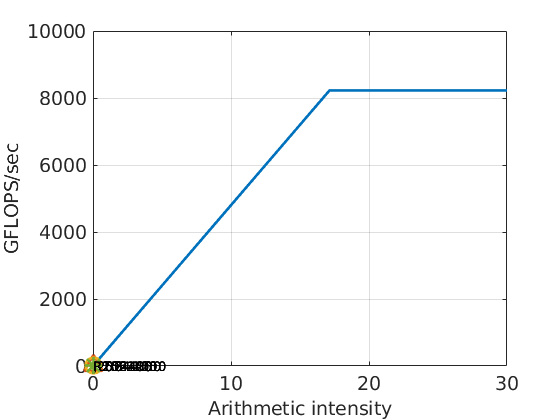
\includegraphics[width=\linewidth]{roofline.png}
	\caption{Roofline.}
	\label{fig:roofline model}
	\end{figure}


The computational performance is not very good. Most of the points are at the hill of the roofline model.
 

%%%% End document
\end{document}
